\icode{E-EME-SI-L3-260625-001}
如图，直角三角形\(\angle ABC\)处在点电荷的电场中，\(\angle B =\) \,\qty{90}{\degree}，\(A\)、\(B\)、\(C\)三点与点电荷在同一平面内，\(O\)为\(AB\)的中点，将一正的点电荷从\(A\)点沿\(AC\)移到\(C\)点，电场力一直做负功，从\(C\)点沿\(CB\)移到\(B\)点，电场力一直做正功，从\(A\)点到\(C\)点克服电场力做的功与\(C\)点到\(B\)点电场力做的功相等。下列图中箭头表示\(C\)点电场的方向，则正确的是\paren[]
    
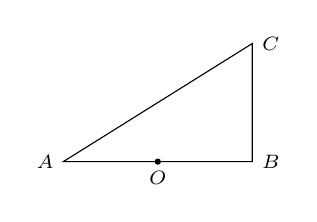
\begin{tikzpicture}[font=\scriptsize]
    \draw (0,0)node[left]{\(A\)}--(2.4,0)node[right]{\(B\)}--(2.4,1.5)node[right]{\(C\)}coordinate(c)--cycle;
    \fill (1.2,0)node[below]{\(O\)} circle(.04);
\end{tikzpicture}

\begin{tikzpicture}[font=\scriptsize,decoration={markings,mark=at position 0.55 with {\arrow{>}}}]
    \begin{scope}
        \draw (0,0)node[left]{\(A\)}--(2.4,0)node[right]{\(B\)}--(2.4,1.5)node[right]{\(C\)}coordinate(c)--cycle;
        \fill (1.2,0)node[above left]{\(O\)} circle(.04);
        \draw[postaction={decorate},blue] (c)--(0,0);
        \node at(1.2,-.5){A};
    \end{scope}
    \begin{scope}[xshift=3.5cm]
        \draw (0,0)node[left]{\(A\)}--(2.4,0)node[right]{\(B\)}--(2.4,1.5)node[right]{\(C\)}coordinate(c)--cycle;
        \fill (1.2,0)node[above left]{\(O\)} circle(.04);
        \draw[postaction={decorate},blue] (c)--(1.2,0);
        \node at(1.2,-.5){B};
    \end{scope}
    \begin{scope}[xshift=7cm]
        \draw (0,0)node[left]{\(A\)}--(2.4,0)node[right]{\(B\)}--(2.4,1.5)node[right]{\(C\)}coordinate(c)--cycle;
        \fill (1.2,0)node[above left]{\(O\)} circle(.04);
        \draw[postaction={decorate},blue] (c)--(1.9,0);
        \node at(1.2,-.5){C};
    \end{scope}
    \begin{scope}[xshift=10.5cm]
        \draw (0,0)node[left]{\(A\)}--(2.4,0)node[right]{\(B\)}--(2.4,1.5)node[right]{\(C\)}coordinate(c)--cycle;
        \fill (1.2,0)node[above left]{\(O\)} circle(.04);
        \draw[postaction={decorate},blue] (c)--(2.4,0);
        \node at(1.2,-.5){D};
    \end{scope}
\end{tikzpicture}
\begin{answer}
    C\quad 提示：
\end{answer}